%% bare_conf.tex
%% V1.4b
%% 2015/08/26
%% by Michael Shell
%% See:
%% http://www.michaelshell.org/
%% for current contact information.
%%
%% This is a skeleton file demonstrating the use of IEEEtran.cls
%% (requires IEEEtran.cls version 1.8b or later) with an IEEE
%% conference paper.
%%
%% Support sites:
%% http://www.michaelshell.org/tex/ieeetran/
%% http://www.ctan.org/pkg/ieeetran
%% and
%% http://www.ieee.org/

%%*************************************************************************
%% Legal Notice:
%% This code is offered as-is without any warranty either expressed or
%% implied; without even the implied warranty of MERCHANTABILITY or
%% FITNESS FOR A PARTICULAR PURPOSE! 
%% User assumes all risk.
%% In no event shall the IEEE or any contributor to this code be liable for
%% any damages or losses, including, but not limited to, incidental,
%% consequential, or any other damages, resulting from the use or misuse
%% of any information contained here.
%%
%% All comments are the opinions of their respective authors and are not
%% necessarily endorsed by the IEEE.
%%
%% This work is distributed under the LaTeX Project Public License (LPPL)
%% ( http://www.latex-project.org/ ) version 1.3, and may be freely used,
%% distributed and modified. A copy of the LPPL, version 1.3, is included
%% in the base LaTeX documentation of all distributions of LaTeX released
%% 2003/12/01 or later.
%% Retain all contribution notices and credits.
%% ** Modified files should be clearly indicated as such, including  **
%% ** renaming them and changing author support contact information. **
%%*************************************************************************


% *** Authors should verify (and, if needed, correct) their LaTeX system  ***
% *** with the testflow diagnostic prior to trusting their LaTeX platform ***
% *** with production work. The IEEE's font choices and paper sizes can   ***
% *** trigger bugs that do not appear when using other class files.       ***                          ***
% The testflow support page is at:
% http://www.michaelshell.org/tex/testflow/



\documentclass[conference]{IEEEtran}
% Some Computer Society conferences also require the compsoc mode option,
% but others use the standard conference format.
%
% If IEEEtran.cls has not been installed into the LaTeX system files,
% manually specify the path to it like:
% \documentclass[conference]{../sty/IEEEtran}





% Some very useful LaTeX packages include:
% (uncomment the ones you want to load)


% *** MISC UTILITY PACKAGES ***
%
%\usepackage{ifpdf}
% Heiko Oberdiek's ifpdf.sty is very useful if you need conditional
% compilation based on whether the output is pdf or dvi.
% usage:
% \ifpdf
%   % pdf code
% \else
%   % dvi code
% \fi
% The latest version of ifpdf.sty can be obtained from:
% http://www.ctan.org/pkg/ifpdf
% Also, note that IEEEtran.cls V1.7 and later provides a builtin
% \ifCLASSINFOpdf conditional that works the same way.
% When switching from latex to pdflatex and vice-versa, the compiler may
% have to be run twice to clear warning/error messages.






% *** CITATION PACKAGES ***
%
%\usepackage{cite}
% cite.sty was written by Donald Arseneau
% V1.6 and later of IEEEtran pre-defines the format of the cite.sty package
% \cite{} output to follow that of the IEEE. Loading the cite package will
% result in citation numbers being automatically sorted and properly
% "compressed/ranged". e.g., [1], [9], [2], [7], [5], [6] without using
% cite.sty will become [1], [2], [5]--[7], [9] using cite.sty. cite.sty's
% \cite will automatically add leading space, if needed. Use cite.sty's
% noadjust option (cite.sty V3.8 and later) if you want to turn this off
% such as if a citation ever needs to be enclosed in parenthesis.
% cite.sty is already installed on most LaTeX systems. Be sure and use
% version 5.0 (2009-03-20) and later if using hyperref.sty.
% The latest version can be obtained at:
% http://www.ctan.org/pkg/cite
% The documentation is contained in the cite.sty file itself.






% *** GRAPHICS RELATED PACKAGES ***
%
\ifCLASSINFOpdf
   \usepackage[pdftex]{graphicx}
  % declare the path(s) where your graphic files are
   \graphicspath{{.}}
  % and their extensions so you won't have to specify these with
  % every instance of \includegraphics
   \DeclareGraphicsExtensions{.pdf,.jpeg,.png}
\else
  % or other class option (dvipsone, dvipdf, if not using dvips). graphicx
  % will default to the driver specified in the system graphics.cfg if no
  % driver is specified.
  % \usepackage[dvips]{graphicx}
  % declare the path(s) where your graphic files are
  % \graphicspath{{../eps/}}
  % and their extensions so you won't have to specify these with
  % every instance of \includegraphics
  % \DeclareGraphicsExtensions{.eps}
\fi
% graphicx was written by David Carlisle and Sebastian Rahtz. It is
% required if you want graphics, photos, etc. graphicx.sty is already
% installed on most LaTeX systems. The latest version and documentation
% can be obtained at: 
% http://www.ctan.org/pkg/graphicx
% Another good source of documentation is "Using Imported Graphics in
% LaTeX2e" by Keith Reckdahl which can be found at:
% http://www.ctan.org/pkg/epslatex
%
% latex, and pdflatex in dvi mode, support graphics in encapsulated
% postscript (.eps) format. pdflatex in pdf mode supports graphics
% in .pdf, .jpeg, .png and .mps (metapost) formats. Users should ensure
% that all non-photo figures use a vector format (.eps, .pdf, .mps) and
% not a bitmapped formats (.jpeg, .png). The IEEE frowns on bitmapped formats
% which can result in "jaggedy"/blurry rendering of lines and letters as
% well as large increases in file sizes.
%
% You can find documentation about the pdfTeX application at:
% http://www.tug.org/applications/pdftex





% *** MATH PACKAGES ***
%
%\usepackage{amsmath}
% A popular package from the American Mathematical Society that provides
% many useful and powerful commands for dealing with mathematics.
%
% Note that the amsmath package sets \interdisplaylinepenalty to 10000
% thus preventing page breaks from occurring within multiline equations. Use:
%\interdisplaylinepenalty=2500
% after loading amsmath to restore such page breaks as IEEEtran.cls normally
% does. amsmath.sty is already installed on most LaTeX systems. The latest
% version and documentation can be obtained at:
% http://www.ctan.org/pkg/amsmath





% *** SPECIALIZED LIST PACKAGES ***
%
%\usepackage{algorithmic}
% algorithmic.sty was written by Peter Williams and Rogerio Brito.
% This package provides an algorithmic environment fo describing algorithms.
% You can use the algorithmic environment in-text or within a figure
% environment to provide for a floating algorithm. Do NOT use the algorithm
% floating environment provided by algorithm.sty (by the same authors) or
% algorithm2e.sty (by Christophe Fiorio) as the IEEE does not use dedicated
% algorithm float types and packages that provide these will not provide
% correct IEEE style captions. The latest version and documentation of
% algorithmic.sty can be obtained at:
% http://www.ctan.org/pkg/algorithms
% Also of interest may be the (relatively newer and more customizable)
% algorithmicx.sty package by Szasz Janos:
% http://www.ctan.org/pkg/algorithmicx




% *** ALIGNMENT PACKAGES ***
%
%\usepackage{array}
% Frank Mittelbach's and David Carlisle's array.sty patches and improves
% the standard LaTeX2e array and tabular environments to provide better
% appearance and additional user controls. As the default LaTeX2e table
% generation code is lacking to the point of almost being broken with
% respect to the quality of the end results, all users are strongly
% advised to use an enhanced (at the very least that provided by array.sty)
% set of table tools. array.sty is already installed on most systems. The
% latest version and documentation can be obtained at:
% http://www.ctan.org/pkg/array


% IEEEtran contains the IEEEeqnarray family of commands that can be used to
% generate multiline equations as well as matrices, tables, etc., of high
% quality.




% *** SUBFIGURE PACKAGES ***
%\ifCLASSOPTIONcompsoc
%  \usepackage[caption=false,font=normalsize,labelfont=sf,textfont=sf]{subfig}
%\else
%  \usepackage[caption=false,font=footnotesize]{subfig}
%\fi
% subfig.sty, written by Steven Douglas Cochran, is the modern replacement
% for subfigure.sty, the latter of which is no longer maintained and is
% incompatible with some LaTeX packages including fixltx2e. However,
% subfig.sty requires and automatically loads Axel Sommerfeldt's caption.sty
% which will override IEEEtran.cls' handling of captions and this will result
% in non-IEEE style figure/table captions. To prevent this problem, be sure
% and invoke subfig.sty's "caption=false" package option (available since
% subfig.sty version 1.3, 2005/06/28) as this is will preserve IEEEtran.cls
% handling of captions.
% Note that the Computer Society format requires a larger sans serif font
% than the serif footnote size font used in traditional IEEE formatting
% and thus the need to invoke different subfig.sty package options depending
% on whether compsoc mode has been enabled.
%
% The latest version and documentation of subfig.sty can be obtained at:
% http://www.ctan.org/pkg/subfig




% *** FLOAT PACKAGES ***
%
%\usepackage{fixltx2e}
% fixltx2e, the successor to the earlier fix2col.sty, was written by
% Frank Mittelbach and David Carlisle. This package corrects a few problems
% in the LaTeX2e kernel, the most notable of which is that in current
% LaTeX2e releases, the ordering of single and double column floats is not
% guaranteed to be preserved. Thus, an unpatched LaTeX2e can allow a
% single column figure to be placed prior to an earlier double column
% figure.
% Be aware that LaTeX2e kernels dated 2015 and later have fixltx2e.sty's
% corrections already built into the system in which case a warning will
% be issued if an attempt is made to load fixltx2e.sty as it is no longer
% needed.
% The latest version and documentation can be found at:
% http://www.ctan.org/pkg/fixltx2e


%\usepackage{stfloats}
% stfloats.sty was written by Sigitas Tolusis. This package gives LaTeX2e
% the ability to do double column floats at the bottom of the page as well
% as the top. (e.g., "\begin{figure*}[!b]" is not normally possible in
% LaTeX2e). It also provides a command:
%\fnbelowfloat
% to enable the placement of footnotes below bottom floats (the standard
% LaTeX2e kernel puts them above bottom floats). This is an invasive package
% which rewrites many portions of the LaTeX2e float routines. It may not work
% with other packages that modify the LaTeX2e float routines. The latest
% version and documentation can be obtained at:
% http://www.ctan.org/pkg/stfloats
% Do not use the stfloats baselinefloat ability as the IEEE does not allow
% \baselineskip to stretch. Authors submitting work to the IEEE should note
% that the IEEE rarely uses double column equations and that authors should try
% to avoid such use. Do not be tempted to use the cuted.sty or midfloat.sty
% packages (also by Sigitas Tolusis) as the IEEE does not format its papers in
% such ways.
% Do not attempt to use stfloats with fixltx2e as they are incompatible.
% Instead, use Morten Hogholm'a dblfloatfix which combines the features
% of both fixltx2e and stfloats:
%
% \usepackage{dblfloatfix}
% The latest version can be found at:
% http://www.ctan.org/pkg/dblfloatfix




% *** PDF, URL AND HYPERLINK PACKAGES ***
%
%\usepackage{url}
% url.sty was written by Donald Arseneau. It provides better support for
% handling and breaking URLs. url.sty is already installed on most LaTeX
% systems. The latest version and documentation can be obtained at:
% http://www.ctan.org/pkg/url
% Basically, \url{my_url_here}.




% *** Do not adjust lengths that control margins, column widths, etc. ***
% *** Do not use packages that alter fonts (such as pslatex).         ***
% There should be no need to do such things with IEEEtran.cls V1.6 and later.
% (Unless specifically asked to do so by the journal or conference you plan
% to submit to, of course. )


% correct bad hyphenation here
\hyphenation{op-tical net-works semi-conduc-tor}

\usepackage{algorithm}
\usepackage{algpseudocode}
%\usepackage{algorithmic}
\usepackage{pifont}
%\usepackage{amsmath}
\usepackage{marginnote}
\usepackage{subfig}

\begin{document}
%
% paper title
% Titles are generally capitalized except for words such as a, an, and, as,
% at, but, by, for, in, nor, of, on, or, the, to and up, which are usually
% not capitalized unless they are the first or last word of the title.
% Linebreaks \\ can be used within to get better formatting as desired.
% Do not put math or special symbols in the title.
\title{Optimizing communications in multi-grid methods using GPUDirect Async}


% author names and affiliations
% use a multiple column layout for up to three different
% affiliations
\author{\IEEEauthorblockN{Elena Agostini}
\IEEEauthorblockA{University "La Sapienza"\\
Rome, Italy\\
Email: elena.ago@gmail.com}
\and
\IEEEauthorblockN{Davide Rossetti}
\IEEEauthorblockA{NVIDIA\\
Santa Clara, CA, USA\\
Email: drossetti@nvidia.com}
\and
\IEEEauthorblockN{Nikolay Sakharnykh\\}
\IEEEauthorblockA{NVIDIA\\
Santa Clara, CA, USA\\
Email: nsakharnykh@nvidia.com}
}
% conference papers do not typically use \thanks and this command
% is locked out in conference mode. If really needed, such as for
% the acknowledgment of grants, issue a \IEEEoverridecommandlockouts
% after \documentclass

% for over three affiliations, or if they all won't fit within the width
% of the page, use this alternative format:
% 
%\author{\IEEEauthorblockN{Michael Shell\IEEEauthorrefmark{1},
%Homer Simpson\IEEEauthorrefmark{2},
%James Kirk\IEEEauthorrefmark{3}, 
%Montgomery Scott\IEEEauthorrefmark{3} and
%Eldon Tyrell\IEEEauthorrefmark{4}}
%\IEEEauthorblockA{\IEEEauthorrefmark{1}School of Electrical and Computer Engineering\\
%Georgia Institute of Technology,
%Atlanta, Georgia 30332--0250\\ Email: see http://www.michaelshell.org/contact.html}
%\IEEEauthorblockA{\IEEEauthorrefmark{2}Twentieth Century Fox, Springfield, USA\\
%Email: homer@thesimpsons.com}
%\IEEEauthorblockA{\IEEEauthorrefmark{3}Starfleet Academy, San Francisco, California 96678-2391\\
%Telephone: (800) 555--1212, Fax: (888) 555--1212}
%\IEEEauthorblockA{\IEEEauthorrefmark{4}Tyrell Inc., 123 Replicant Street, Los Angeles, California 90210--4321}}




% use for special paper notices
%\IEEEspecialpapernotice{(Invited Paper)}




% make the title area
\maketitle

% As a general rule, do not put math, special symbols or citations
% in the abstract
\begin{abstract}

HPGMG is an HPC benchmark based on geometric multi-grid methods.
%
A multi-grid solver works on levels of different sizes so that the amount of
computation and communication varies a lot within the same application.
% 
%At certain levels, to increase performance, some stages are executed on the
%low-latency processor (CPU). Similarly, data can be dinamically compacted
%onto a subset of the compute nodes.

NVIDIA has developed a CUDA version of HPGMG-FV (Finite Volume) where,
according to a threshold, finer (higher) levels are computed on the GPU
while coarser (lower) levels on the CPU: this hybrid scheme takes advantage
of each processor strengths.
% 
During the HPGMG-FV execution there are three main communication
phases: boundaries exchange (among a variable number of cluster nodes),
interpolation (lower to higher level) and restriction (higher to lower
level). By default communications use the Message Passing Interface (MPI).

GPUDirect Async is a new technology introduced by NVIDIA in CUDA 8.0 which
allows mutual direct control between the GPU and the interconnect device, a
Mellanox Infiniband HCA in our case.
 
In this paper, we propose two optimized communication schemes involving the
GPUDirect Async technology, where the burden of the communication is
off-loaded onto the GPU itself.
% 
When running a properly modified version of HPGMG-FV, where Async
technology is used for only those aforementioned communication phases, we
measured a communication performance increase of up to 13\%.

\end{abstract}

% no keywords




% For peer review papers, you can put extra information on the cover
% page as needed:
% \ifCLASSOPTIONpeerreview
% \begin{center} \bfseries EDICS Category: 3-BBND \end{center}
% \fi
%
% For peerreview papers, this IEEEtran command inserts a page break and
% creates the second title. It will be ignored for other modes.
\IEEEpeerreviewmaketitle



\section{Introduction}\label{sec:introduction}
Linear solvers are probably the most common tool in scientific computing applications and can be divided in two basic classes: \emph{direct} and \emph{iterative}.
% Direct methods are usually robust, but have additional computational complexity and memory capacity requirements, while iterative solvers require minimal memory overhead and feature better computational complexity. 
\emph{Multi-grid} methods are iterative methods that can deliver linear complexity by solving elliptic PDEs $Ax=b$ using a hierarchical approach, i.e. the solution to an hard problem (finer grid of elements) is expressed as solution to an easier problem (coarser grid of element).
There are two different types of \emph{Multi-grid} methods: algebric multi-grid (\emph{AMG}), where operator A is a sparse matrix, and geometric multi-grid (\emph{GMG}), where operator A is a stencil\footnote{Stencil codes are a class of iterative kernels which update array (generally a 2- or 3-dimensional regular grid) elements (cells) according to some fixed pattern, called stencil. The state of a cell in the next time step can be deduced from its own previous state and the states of the cells in its neighborhood.
}. While AMG method is a more general approach using an arbitrary graph, GMG method is more efficient on structured problems, since is can take advantage of the additional information from the geometric representation of the problem.

An example of GMG is HPGMG \cite{HPGMG}, an HPC benchmarking effort developed by Lawrence Berkeley National Laboratory. In particular, HPGMG-FV solves variable-coefficient elliptic problems on isotropic Cartesian grids using the finite volume method (FV) \cite{finitevolume} and Full Multigrid (FMG) \cite{fullmultigrid}. It supports high-order discretizations, and is extremely fast and accurate; in case of multi-process execution, the workload is fairly distributed among processes because, in order to improve the parallelization, each problem level is divided into several same-size boxes.

NVIDIA improved the HPGMG-FV implementation \cite{HPGMG_NVIDIA} using a hybrid solution (involving both CPU and GPU), achieving a great enhancement in performances. In Section \ref{sec:hpgmg_cuda} we explain the most important changes carried out by NVIDIA useful to understand the rest of the paper.

Considering the NVIDIA hybrid implementation, in case of multi-GPU (multi-process) execution, communications play an important role in the algorithm. Section \ref{sec:gpudirect_async_hpgmg}, focus on the communication enhancement obtained by the use of GPUDirect Async, a new technology introduced by NVIDIA in CUDA 8.0 (see Section \ref{sec:gpudirect_async})


\section{HPGMG-FV with CUDA}\label{sec:hpgmg_cuda}

At the core of every multi-grid solver there is a V-cycle (Figure \ref{fig:hpgmg_vcycle}) computation pattern: starting from the finest structured grid, where a smoothing operation is applied to reduce high-frequency errors, the residual is calculated and propagated to the coarser grid. This process is repeated until the bottom level is reached, at which point the coarsest problem is solved directly, and then the solution is propagated back to the finest grid. The V-cycle is mainly dominated by the smoothing (GSRB smoother in our case), and residual operations at the top levels. These are usually 3D stencil operations on a structured grid.

\begin{figure}[h]
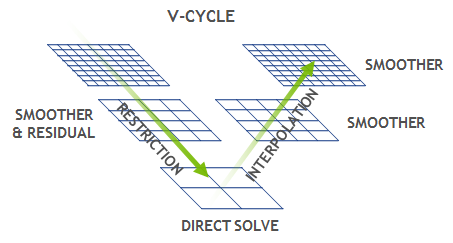
\includegraphics[scale=0.7]{hpgmg_v_cycle.png}
\caption{V-Cycle}
\label{fig:hpgmg_vcycle}
\end{figure}

HPGMG-FV implements an F-cycle, which starts at the bottom of the multi-grid hierarchy and performs multiple V-cycles, gradually adding finer levels. 
HPGMG-FV takes as input the number and the $log_2(size)$ of the finest level boxes, calculating the level total size; then it obtains the size of all the other (smaller) levels.
The F-cycle is considered a state-of-the-art in multi-grid methods and converges much faster than a conventional V-cycle.

NVIDIA analyzed the difference among levels in an F-Cycle: Top (fine) levels have lots of grid points and can run efficiently on throughput-oriented parallel architectures like GPUs, while bottom (coarse) levels will be latency limited on a GPU because there is not enough work to make efficient use of all the parallel cores. During an F-Cycle, coarse levels are visited progressively more often than the fine levels therefore their cost is significant in an F-Cycle. For those reasons, coarse grids are better suited for latency-optimized processors like CPUs.
Thus, for optimal performance, an hybrid scheme is required to guarantee that each level is executed on the suitable architecture: if the size of a level is over a certain threshold (empirically set to 10000 elements), then it runs on GPU, otherwise on CPU (Figure \ref{fig:hpgmg_fcycle}).

\begin{figure}[h]
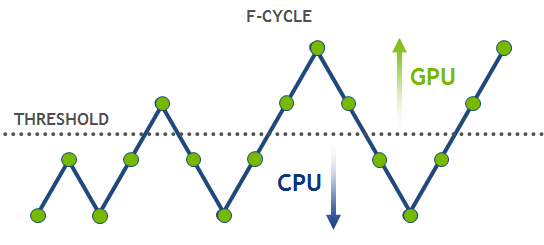
\includegraphics[scale=0.6]{hpgmg_f_cycle.png}
\caption{F-Cycle with CPU-GPU threshold}
\label{fig:hpgmg_fcycle}
\end{figure}
 
To enable GPU accelleration, the simplest way was to add corresponding GPU kernels for low-level stencil operators and update memory allocations using \textit{cudaMallocManaged()} instead of \textit{malloc()}, in order to use Unified Memory \cite{unifiedmemory} for memory used by GPU only, and use host pinned memory if it must be used by both CPU and GPU (i.e. communication buffers).

In Figure \ref{fig:hpgmg_levels} there is a simplified operations timeline in case of coarse level (CPU) to fine level (GPU) and again coarse level (CPU).

\begin{figure}[h]
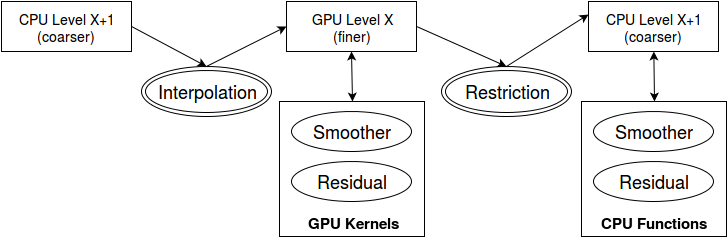
\includegraphics[scale=0.35]{hpgmg_levels.png}
\caption{F-Cycle: moving from a coarse level to a finer level and then go back to the coarse level}
\label{fig:hpgmg_levels}
\end{figure}

In Figure \ref{fig:hpgmg_ornl_bench} we report the enhancement obtained by NVIDIA using the hybrid solution in a benchmark on the ORNL Titan supercomputer \cite{ornl}. For further details, please refer to \cite{HPGMG_NVIDIA}

\begin{figure}[h]
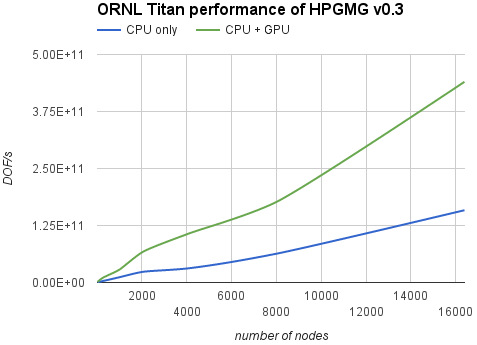
\includegraphics[scale=0.7]{hpgmg_ornl_titan_perf_cuda.png}
\caption{Performance of GPU-accelerated HPGMG on the ORNL Titan supercomputer. Results obtained by Sam Williams from Lawrence Berkeley National Lab.}
\label{fig:hpgmg_ornl_bench}
\end{figure}


\subsection{Communication periods}\label{sec:hpgmg_cuda_communications}

As described in Section \ref{sec:hpgmg_cuda}, in \emph{Multi-grid} methods the smoother is a stencil and in case of HPGMG the tasks for each process are:
\begin{enumerate}
%local grid?
\item Pack: copy grid boundaries data inside send buffers
\item Send: distribute boundaries to the other processes
\item Interior Compute: work on interior grid elements
\item Receive: receive boundaries from the other processes
\item Unpack: copy received data into the grid boundaries
\end{enumerate}

Therefore, in case of multi-GPU execution the smoother must exchange the boundary regions with the other processes (\emph{intra-level} communication). 
On the contrary, (Figure \ref{fig:hpgmg_levels}) restriction and interpolation play a role in case of moving from a level to another (\emph{inter-level} communication).
\emph{inter-level} exchanges play a bigger role at scale where we do consolidation of 8N to N processes (so we have lots of data moved around)

\subsubsection{Exchange Boundaries}

This function implements the boundary region exchange doing a \{pack\}, \{send\}, \{interior\_compute\}, \{receive\}, \{unpack\} sequence among processes working on the same level. See Algorithm \ref{algo:exchange_boundaries} for the pseudo-code.

\begin{algorithm}
\small
\caption{Exchange Boundaries function}
\label{algo:exchange_boundaries}
\begin{algorithmic}[1]
\For{$i$ = 1 to PROCESSES }
\State cudaMallocHost(sendBuffers$[i]$)
\State cudaMallocHost(receiveBuffers$[i]$)
\EndFor
\State ...
\Function{exchangeBoundaries()}{} \label{alg:b}
	\For{$i$ = 1 to PROCESSES }
		\State MPI\_Irecv(receiveBuffers$[i]$, \&reqs\_recv$[i]$)    
	\EndFor
	\State cuda\_pack(sendBuffers)
	\State cudaDeviceSynchronize()
	\For{$i$ = 1 to PROCESSES }
		\State MPI\_Isend(sendBuffers$[i]$)    
	\EndFor
	\State cuda\_interior\_compute(localBuffers)
	\State MPI\_Waitall(reqs\_recv)
	\State cuda\_unpack(receiveBuffers)
\EndFunction
\end{algorithmic}
\end{algorithm}

A \textit{cudaDeviceSynchronize()} is required between the CUDA kernel pack operation and the \textit{MPI\_Isend()} to guarantee correctly updated \textit{sendBuffers}.
The \textit{exchangeBoundaries()} is the most used communication function during an HPGMG-FV execution.

\subsubsection{Restriction}

This function occurs when moving from a finer level to a coarser level; in case of GPU-to-CPU level, it is quite similar to \textit{exchangeBoundaries()}: GPU kernels works on \textit{sendBuffers}, then a \textit{cudaDeviceSynchronize()} is needed before the \textit{MPI\_Isend()}. Moreover, if the coarsest level is on CPU, an additional \textit{cudaDeviceSynchronize()} is required because GPU kernels are launched asynchronously and we need to guarantee completion before we start CPU tasks.

\subsubsection{Interpolation}

It occurs when moving from a coarser level to a finer level. It requires a \textit{cudaDeviceSynchronize()} before the \textit{MPI\_Isend()} but it doesn't needs to synchronize if the coarsest level is on CPU because CPU tasks are synchronous and they will be completed before we launch GPU kernels.

Although communications are not the most expensive part of the algorithm, profiling the GPU levels execution we noticed that:

\begin{itemize}
\item the CPU launched a lot of CUDA kernels for residual and smoothing and each kernel launch required a lot of time, leaving sometime the GPU idle, waiting for an other kernel
\item the high number of \textit{cudaDeviceSynchronize()} slowed the performances 
\end{itemize}

To hide the kernel launches and remove as many   \textit{cudaDeviceSynchronize()} as possible, we used GPUDirect Async (see Section \ref{sec:gpudirect_async}) to improve performances of all the communications periods.

In Figure \ref{fig:timeline_mpi} there is a simplified timeline to clarify how \textit{exchangeBoundaries()}, \textit{restriction()} and \textit{interpolation()} are used during a GPU level processing.

\begin{figure}[h]
\centering
\includegraphics[scale=0.25]{timeline_mpi.png}
\caption{Synchronous \textit{exchangeBoundaries()} timeline}
\label{fig:timeline_mpi}
\end{figure}

\section{GPUDirect Async}\label{sec:gpudirect_async}

GPUDirect \cite{GPUDirect} is a family of technologies aimed at optimizing data movement respectively among GPUs (P2P) and with third-party devices (RDMA). In particular, GPUDirect RDMA reduces latency and improves bus utilization by enabling a direct data path over the PCI Express (PCIe) bus between the GPU and a third-party device, in our case a network interface controller (NIC).

GPUDirect Async is a new GPUDirect technology introduced by NVIDIA in CUDA 8.0; it allows mutual direct control between the GPU and the third party device, a recent generation Infiniband HCA in our case.

Although an in-depth explaination of the GPUDirect Async implementation is beyond the scope of this paper, in the following we will breafly describe how it works and how it can be leveraged in HPGMG-FV.
With Async the GPU is able to trigger communications on HCA, while at the same time HCA is able to unblock CUDA tasks; the CPU is only needed to prepare and queue both the compute and communication tasks on GPU. 
%
More specifically:
\begin{itemize}

\item The CPU allocates communication buffers (device or host pinned memory).

\item It maps some HCA specific data structures, like command queues (IB
  Verbs QPs) and completion queues (IB Verbs CQs), onto the GPU by using
  \textit{cuMemHostRegister()}.

\item Prepares the send/receive requests descriptors.

\item Converts those descriptors into a sequence of basic operations to be
  executed by the GPU, for example by the GPU front-end unit which is in
  charge of the CUDA stream abstraction. Examples of those operations are:

  \begin{itemize}
  \item Writing an HW mailbox register onto the HCA, i.e. ringing the HCA doorbell.
  \item Triggering a pre-launched CUDA kernel.
  \item Waiting (polling) for communication task completion (IB Verbs CQ entries, or CQEs).
  \end{itemize}

\end{itemize}

For example, after having prepared and queued all the necessary tasks onto
the GPU, the CPU can go back and do other useful work.
% 
By leveraging this mechanism a whole parallel computation phase can be
offloaded onto a CUDA stream.
%
Still when necessary, the CPU can query the CUDA stream for the status of
the outstanding operations.
% 
The same mechanism is expected to be useful to efficiently scale up in
combination with a low performance CPU, effectively removing its
cohordinating work from the critical path.

\begin{figure}[h]
\centering
\includegraphics[scale=0.35]{gpudirectasync.png}
\caption{GPUDirect Async Software stack}
\label{fig:gpudirectasync}
\end{figure}

The GPUDirect software stack (Figure \ref{fig:gpudirectasync}) comprises:

\subsubsection{libmlx5}(Vendor/device specific)
\emph{libmlx5} is a low-level device driver for Mellanox Connect-IB InfiniBand host channel adapters (HCAs). This allows userspace processes to access Mellanox HCA hardware directly with low latency and low overhead. The standard implementation has been extended for needs of GPUDirect Async.

\subsubsection{libibverbs}(Verbs APIs)
\emph{libibverbs} library implements the OpenFabrics Infiniband Verbs API. The standard implementation has been extended with new Verbs specific to GPUDirect Async.

\subsubsection{LibGDSync}(NVIDIA open-source)
Developed by NVIDIA, it consist of a set of hybrid APIs where both IB Verbs and CUDA GPU stream are merged. It is responsible to create IB tracking data structures respecting the constraints of GPUDirect Async, to register host memory when needed, to post send instructions and completion waiting directly on the GPU stream.
 
\subsubsection{LibMP}(NVIDIA open-source)
It is at the top level and is a messaging library (similar to MPI) developed as a tecnology demostrator to easily deploy the GPUDirect Async technology on MPI applications.
It leverages LibGDSync APIs and offer basic communications like \textit{mp\_isend\_on\_stream()}, \textit{mp\_wait\_on\_stream()}, \textit{mp\_iput\_on\_stream()}, etc.. 

In addition to the Stream Async communication model previously described,
where communications are synchronous to the CUDA streams, in this paper we are
going to explore a \textit{kernel-initiated} model, where the Simultaneous
Multiprocessors (SMs), which are in charge of executing the CUDA kernels,
can directly issue communication primitives, i.e. sending messages and
waiting for completions.
%
% 
%The former is more adapt to a coarse-grained communication pattern and
%can leverage strong memory consistency guarantees, while the latter is more
%akin to fine-grained communications

%GPUDirect Async has two different asynchronous modes:
%\begin{enumerate}
%\item Stream Async: to instruct a GPU stream, as explained before
%\item kernel-initiated: to launch a single CUDA kernel in which communications and computations can be done by the same kernel within the code, using send/receive $\_\_device\_\_$ primitives\\
%\end{enumerate}

In the following sections, we will show that kernel-initiated mode can be faster than Stream Async mode, i.e. by allowing kernel fusion techniques thereby exposing more concurrency to the highly parallel GPU HW units. The downside of it is that it is more complicated to use, mainly because the programmer needs to manually schedule different sub-tasks (send, receive or compute) to separate CUDA kernel thread blocks respecting the constraints of the algorithm.

%%We are working on a more detailed and complete paper about the GPUDirect Async implementation.


\section{Asynchronous communications}\label{sec:gpudirect_async_hpgmg}

We tried both the asynchronous modes in HPGMG-FV, to evaluate performances considering execution times of GPU levels only.

\subsection{Stream Async mode}

See Algorithm \ref{algo:exchange_boundaries_async} for the \textit{exchangeBoundariesAsync()} pseudo-code.

\begin{algorithm}
\small
\caption{Exchange Boundaries Stream Async function}
\label{algo:exchange_boundaries_async}
\begin{algorithmic}[1]
\For{$i$ = 1 to PROCESSES }
\State cudaMallocHost(sendBuffers$[i]$)
\State cudaMallocHost(receiveBuffers$[i]$)
\EndFor
\State ...
\Function{exchangeBoundariesStreamAsync(stream)}{} \label{alg:a}
	\For{$i$ = 1 to PROCESSES }
		\State mp\_irecv(receiveBuffers$[i]$, \&receiveDescriptors$[i]$)    
	\EndFor
	\State cuda\_pack(sendBuffers, stream)
	\For{$i$ = 1 to PROCESSES }
		\State mp\_isend\_on\_stream(sendBuffers$[i]$, \&sendDescriptors$[i]$, stream)    
	\EndFor
	\State cuda\_interior\_compute(localBuffers)
	\State mp\_wait\_all\_on\_stream(receiveDescriptors)
	\State cuda\_unpack(receiveBuffers)
	\State mp\_wait\_all\_on\_stream(sendDescriptors)
\EndFunction
\end{algorithmic}
\end{algorithm}

The \textit{cudaDeviceSynchronize()} between \textit{cuda\_pack()} and \textit{mp\_isend\_on\_stream()} function is no more required. The GPU stream will:

\begin{enumerate}
\item Write on \textit{sendBuffers} using the \textit{cuda\_pack()} kernel
\item Post the send requests
\item Execute the \textit{cuda\_interior\_compute()} kernel
\item Wait the receive completion
\item Read the received data (\textit{receiveBuffers}) with the \textit{cuda\_unpack()} kernel
\end{enumerate}

Similar considerations can be done for \textit{restriction()} and \textit{interpolation()} functions.

Stream Async is used only if the level is a GPU level: this means that only a \textit{cudaDeviceSynchronize()} is needed during the \textit{restriction()} function from the last GPU (higher) level to the first CPU (lower) level. During GPU levels, CPU can launch all the CUDA kernels without waiting, hiding the kernel launches times (Figure \ref{fig:timeline_async}).

\begin{figure}[h]
\centering
\includegraphics[scale=0.3]{timeline_async.png}
\caption{\textit{exchangeBoundariesStreamAsync()} timeline showing respectively the CPU and the GPU tasks.}
\label{fig:timeline_async}
\end{figure}



\subsection{kernel-initiated mode}

\begin{figure*}
%\includegraphics[width=\textwidth]{hpgmg_gpu.png}
\subfloat[\textit{exchangeBoundariesKernelInitiated()} timeline.]{\includegraphics[width=2.8in]{timeline_gpu.png}}
\hfil
\subfloat[In the cuda\_compute\_exchange\_kernel(), thread blocks are assigned different tasks.]{\includegraphics[width=4.1in]{hpgmg_gpu.png}}
\caption{kernel-initiated mode}
\label{fig:gpu_initited}
\end{figure*}

From the CPU point of view, the algorithm \ref{algo:exchange_boundaries_gpu}
is extremely simple (Figure \ref{fig:gpu_initited}.
% 
The \textit{exchangeBoundariesKernelInitiated()} function basically
prepares the send/receive descriptors and launches a single \textit{fused}
CUDA kernel (\textit{cuda\_compute\_exchange\_kernel}) which combines all
the tasks described in algorithm \ref{algo:exchange_boundaries}.

% will fuse, as much as possible, all the \textit{exchangeBoundaries()} operations (see Algorithm \ref{algo:exchange_boundaries_gpu}).

\begin{algorithm}
\small
\caption{Exchange Boundaries kernel-initiated function}
\label{algo:exchange_boundaries_gpu}
\begin{algorithmic}[1]
\For{$i$ = 1 to PROCESSES }
\State cudaMallocHost(sendBuffers$[i]$)
\State cudaMallocHost(receiveBuffers$[i]$)
\EndFor
\State ...
\Function{exchangeBoundariesKernelInitiated()}{}
	\For{$i$ = 1 to PROCESSES }
		\State mp\_irecv(receiveBuffers$[i]$, \&receiveDescriptors$[i]$)    
	\EndFor
	\For{$i$ = 1 to PROCESSES }
		\State mp\_isend\_prepare(\&sendDescriptors$[i]$)
	\EndFor
	\State cuda\_compute\_exchange\_kernel(receiveDescriptors, sendDescriptors)
	\State mp\_wait\_all\_on\_stream(sendDescriptors)
\EndFunction
\end{algorithmic}
\end{algorithm}

The complexity is moved to \textit{cuda\_compute\_exchange\_kernel()} which
in a sense employs both tasks (different blocks deal with different tasks)
and data (threads in the same block cooperatively work on the same task)
parallelism in the same kernel.

According to previous observations about the HPGMG-FV smoother, we can
distringuish three different groups of independent operations:
%\begin{itemize}
\lbrack pack, send\rbrack,
\lbrack interior compute\rbrack,
\lbrack receive, unpack\rbrack. 
%\end{itemize}
% 
The idea is to assign these tasks to the different blocks of a single CUDA
kernel.
%
Basically, the \textit{cuda\_compute\_exchange\_kernel()} needs $N+M+1$
blocks in a mono-dimensional grid, where N is the number of blocks required
by the \textit{cuda\_pack()} and \textit{cuda\_interior\_compute()} and M
is the number of blocks required by \textit{cuda\_unpack()} plus 1 block,
used to receive data as explained in Figure \ref{fig:gpu_initited}.
% 
Atomic memory operations are used to pick each thread block
\footnote{There is no guarantee about the order blocks are scheduled by the
  GPU HW.} and to assign it to the right tasks in a way to avoid
dead-locks.

Receiving is a time critical task, so the first \textit{receiver} thread
block is used to wait for incoming messages; in particular each thread
\textit{polls} on the receive completion queue associated to each remote
node.
% 
All the \textit{sender} blocks from the second to the $N+1$-th are assigned
to the \lbrack pack, send\rbrack group of operations plus the \lbrack
interior compute\rbrack.
% 
Finally the remaining M \textit{unpacker} blocks wait for the
\textit{receiver} block to signal that all incoming data has been received,
before unpacking that data.


\begin{figure}[h]
\includegraphics[scale=0.4]{global_lock.png}
\caption{Global Lock among kernel blocks}
\label{fig:global_lock}
\end{figure}

An inter-block barrier scheme is used to synchronize the \textit{receiver}
and the \textit{unpacker} blocks, as explained in Figure
\ref{fig:global_lock}.
% 
Thread0 of each \textit{unpacker} block waits for the Thread0 of the
\textit{receiver} block to set a global memory variable to 1, while the
remaining threads move to the \textit{\_\_syncthreads()} barrier.
%
When this happens (after the receive completion), all the Thread0 in the
\textit{receiver} blocks will reach the matching \textit{\_\_syncthreads()}
barrier and then start to unpack the received data.

When using kernel-initiated mode, to avoid dead-locks the \textit{receiver}
task must not prevent the \textit{sender} task from starting or
progressing.
% 
For example, on a 15 SMs GPU like the NVIDIA K40, if the first one is running the
\textit{receiver} task and the others 14 are busy running the
\textit{unpacker}, the \textit{sender} task will never start.

\section{Benchmarks and results}

As described in Section \ref{sec:hpgmg_cuda}, HPGMG-FV takes as input the size and number of the boxes in the highest level; during our benchmarks we used 8 boxes varying the size in \lbrack 4,5,6,7\rbrack.
According to Section \ref{sec:hpgmg_cuda}, the threshold size used during NVIDIA tests was 10000; considering 4 as minimun $log_2$ size for boxes, this means that the 3 smallest levels are always executed on CPU and all the others on GPU.

We tried different threshold values (i.e. changing the number of GPU levels for each execution) during our asynchronous benchmarks but we found that the best values is always 10000.

\subsection{Two node benchmarks}
\label{sec:two-nodes}

For the first round of benchmarks we used two standard 2U Xeon based
servers, each one with a Mellanox dual-port FDR Connect-IB HCA and a single
Tesla K40m (boost clocks set to 875 MHz), running RHEL 6.6 and a
pre-release version of the GPU display driver.
% 
In Figure \ref{fig:gain_ivy} the Y axis shows the performance increase (the
larger the better) of the GPU levels only for both Stream Async and
kernel-initiated mode over the standard MPI mode. 
%
The bigger is the box size, the more performance gain decreases, because
communication message size grows with the box size, so therefore
overheads become less important.
% 
Here we also note the the kernel-initiated mode always wins over the
Stream Async one.

\begin{figure}[h]
\centering
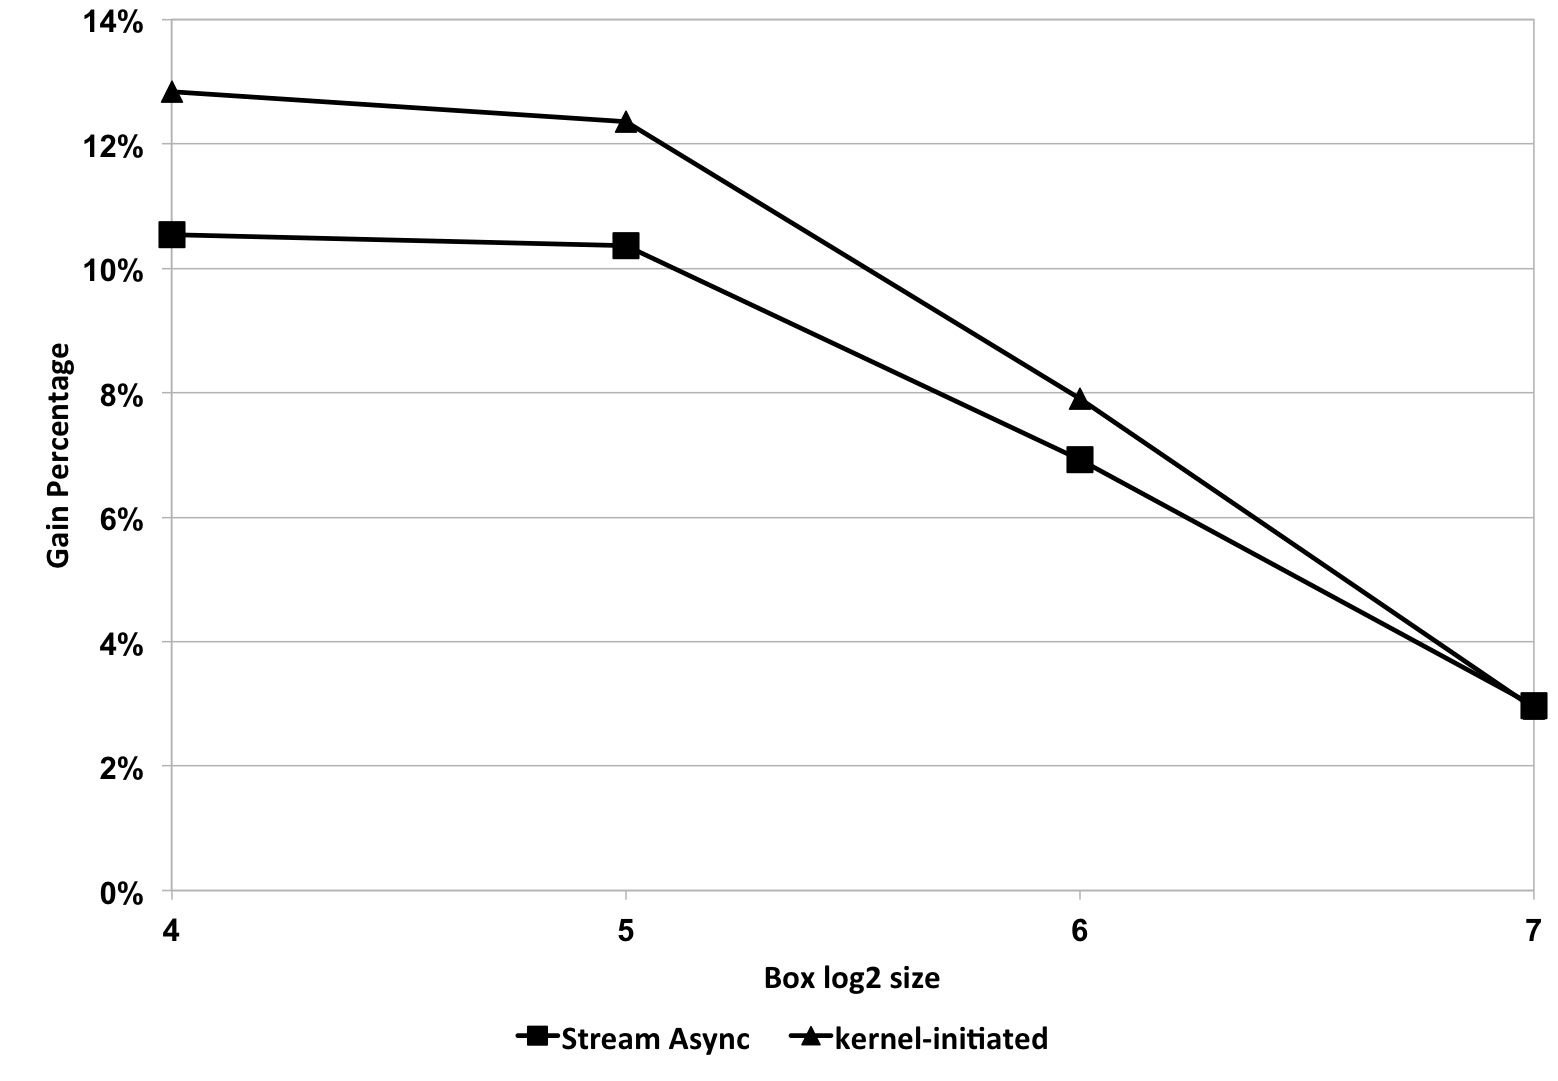
\includegraphics[scale=0.3]{gain_ivy.png}
\caption{2 processes, Asynchronous time gain, 2U Xeon Servers}
\label{fig:gain_ivy}
\end{figure}

\subsection{Scaling up}

For this second benchmark, we used the Wilkes HPC cluster at the Cambridge
University, UK)\cite{wilkes}.
% 
The system consists of 128 Dell T620 servers, 256 NVIDIA Tesla K20c GPUs
interconnected by 256 Mellanox Connect IB cards.
% 
For technical reasons we were only able to use up to 16 cluster nodes,
with one GPU each.
%
Figure \ref{fig:gain_wilkes} plots the performance increase on two nodes,
i.e. the same setup as in the previous section.

\begin{figure}[h]
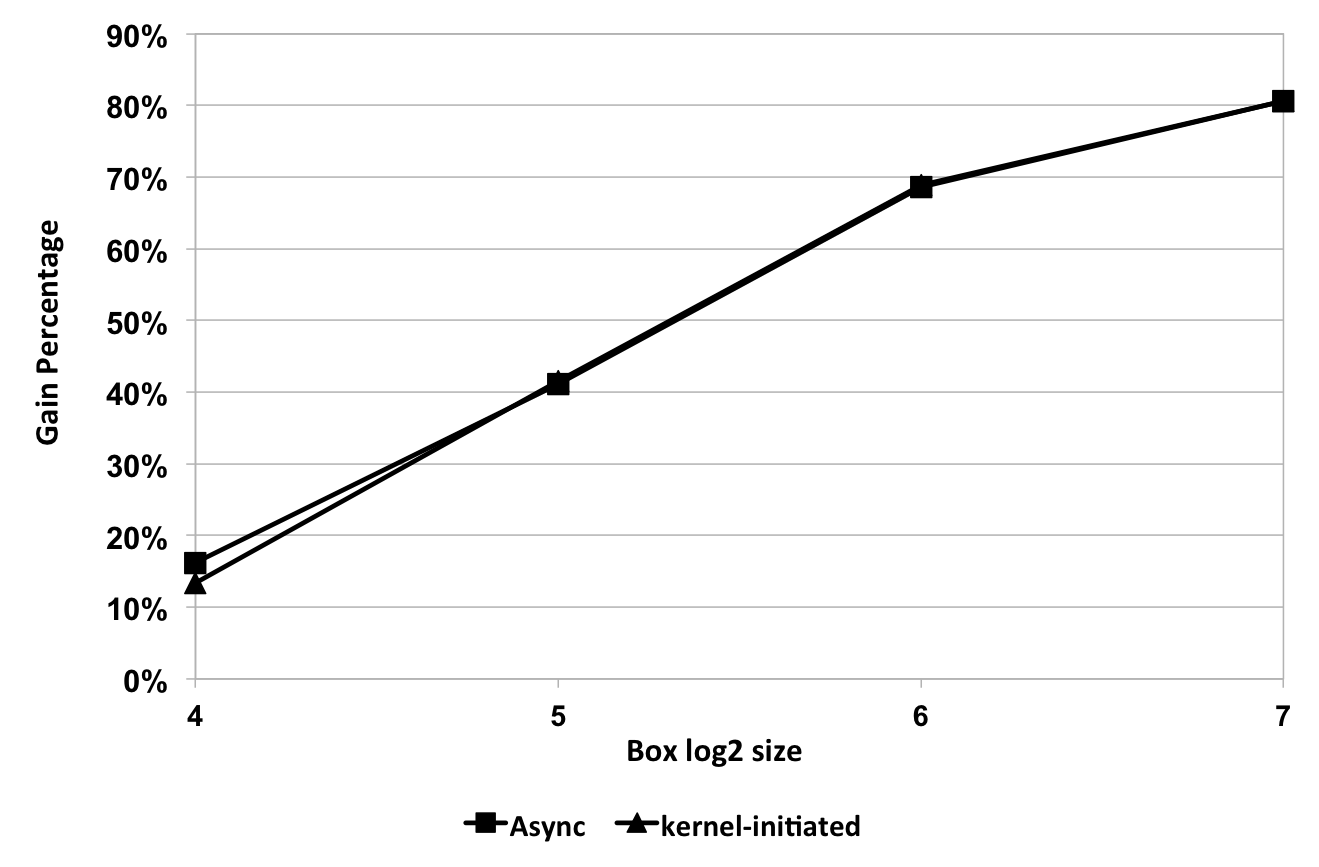
\includegraphics[scale=0.4]{gain_wilkes.png}
\caption{HPGMG-FV, 2 processes, Async and kernel-initiated mode gain over
  default MPI communications, Wilkes HPC}
\label{fig:gain_wilkes}
\end{figure}

For small sizes both Async and kernel-initiated modes show a similar
performance, with Async being marginally better.
% 
Instead the substantial gain obtained (80\% over standard MPI) for box
size 7 with Async modes for large sizes was somehow unexpected.
%
That has been traced back to a subperforming implementation of the Unified
Memory manager in the pre-release GPU driver installed on the Wilkes
cluster
\footnote{A software update will soon be deployed to fix the Unified Memory
  performance on the Wilkes cluster.}.
%
On the contrary, execution times of the Async versions were similar
to the first round of benchmarks in section ~\ref{sec:two-nodes}.
%
Irrespective of the particular contingency, this shows an additional
benefit of Async, i.e. it makes the application less sensitive to
host software overheads.

When scaling up on 16 nodes (Figure \ref{fig:gain_wilkes16}), for the
smallest size we observed 50\% better performance for kernel-initiated mode
over Async mode.
% 

This is expected given the HPGMG-FV communication pattern, where each GPU
can potentially exchange data with up to 15 other GPUs.
%
In kernel-initiated mode different threads deal with different communication
tasks, e.g. each thread of a dedicated CUDA thread block is used to
initiate message sends to the different destinations.



\begin{figure}[h]
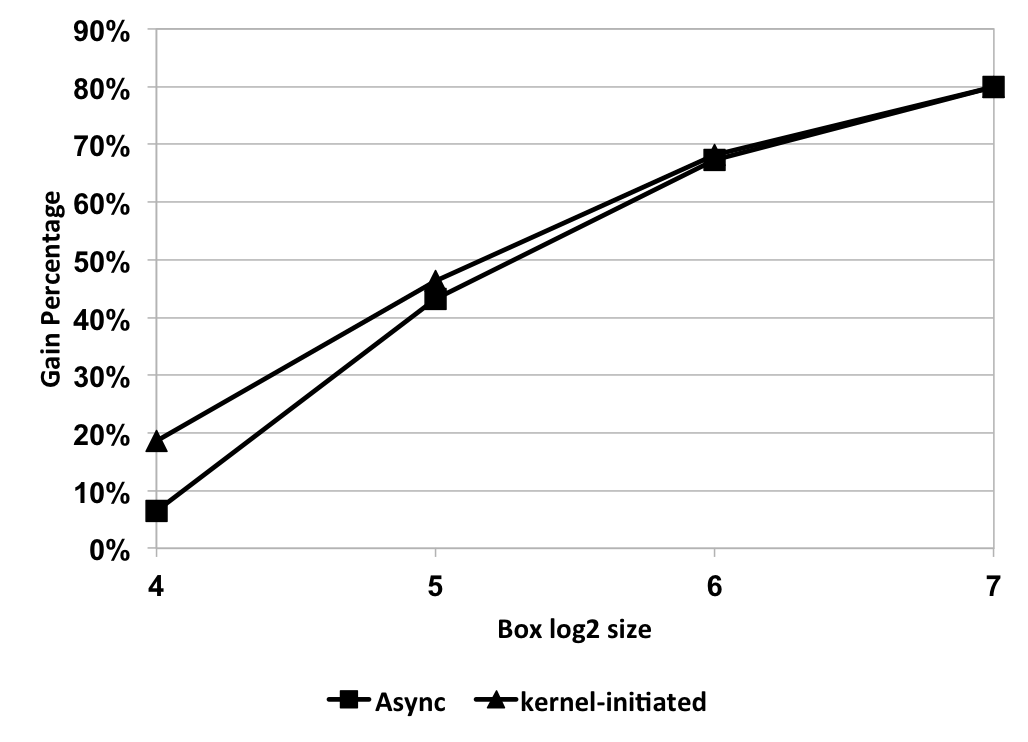
\includegraphics[scale=0.5]{gain_wilkes16.png}
\caption{HPGMG-FV, 16 processes, Async and kernel-initiated mode gain over
  default MPI communications}
\label{fig:gain_wilkes16}
\end{figure}

%Finally, in Figure \ref{fig:gain_driver} there is the time gain of the asynchronous implementations using NVIDIA internal driver respect to the public 361.62 driver.

%\begin{figure}[h]
%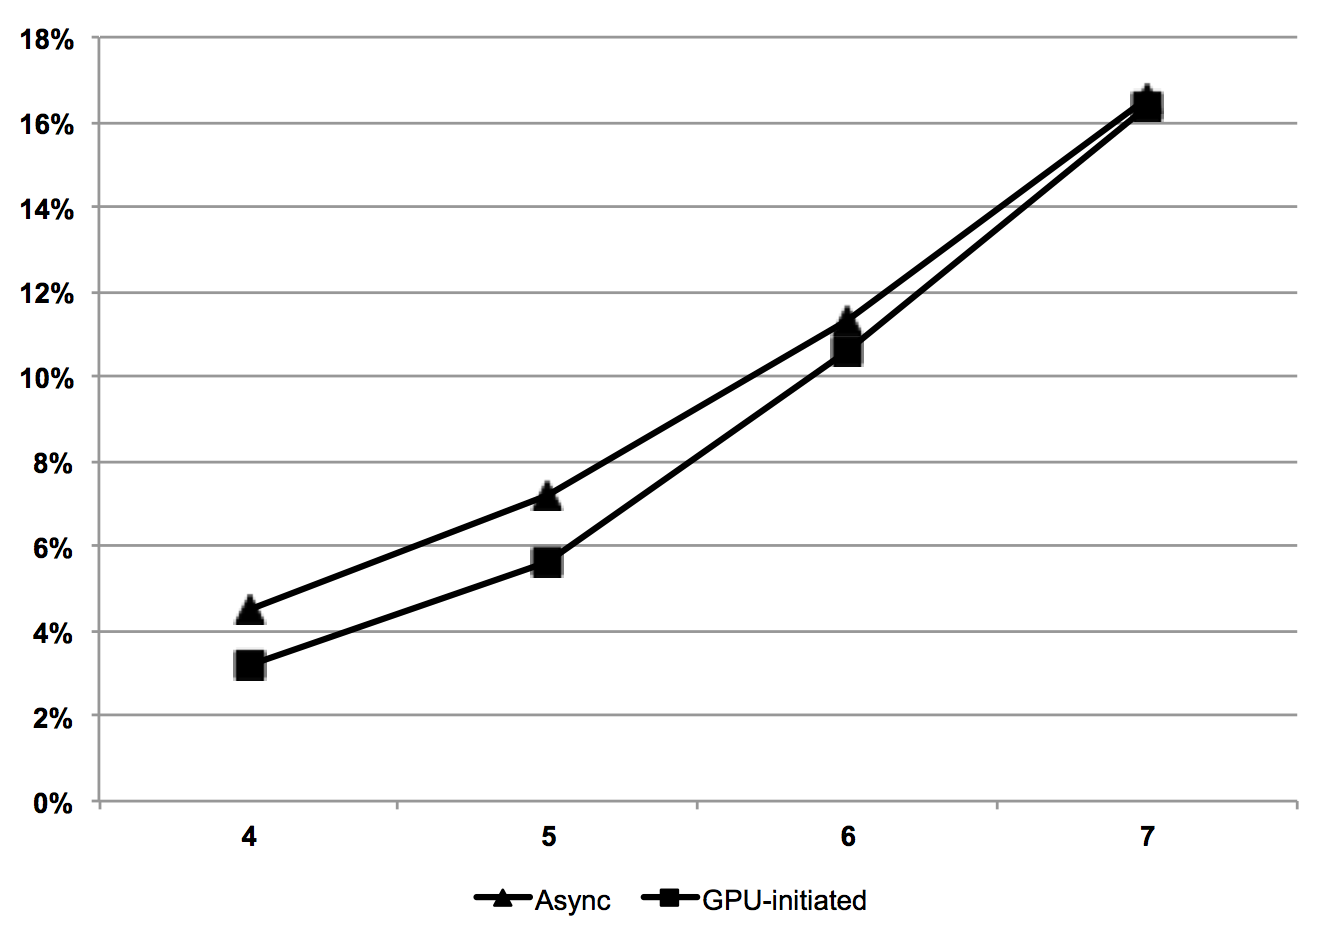
\includegraphics[scale=0.4]{gain_driver.png}
%\caption{HPGMG-FV, 2 processes, Async modes gains over MPI, NVIDIA internal driver on 361.62 driver}
%\label{fig:gain_driver}
%\end{figure}

%Recently NVIDIA updated the display driver in CUDA 8.0 RC to the 361.77 version; we are waiting for the driver update on Wilkes HPC to perform the same benchmark again.

%% \subsection{2D Stencil}

%% To avoid the UVM issues, we tested asynchronous communications using a synthetic two dimensional stencil code.
%% %Description from README in peersync/src/2dstencil
%% Basically, our implementation simulates computation on a 2D stencil distributed across a 2D grid of processes. The computation is a simple average where the value of an element in the current iteration depends on the values of its neighboring elements (1-cell stencil) from the previous iteration. The near-neighbor exchange involves transferring the outermost most layer of the data grid between neighboring processes. There are two data grids, u and v, where one is computed from the other, alternatingly, in each iteration. This is modeled after the presence of multiple components in real science problems that affect each other over time, for example velocity and stress in seismic modeling codes.\\

%% As in HPGMG, we can distringuish three different groups of independent operations: \lbrack pack, send\rbrack, \lbrack interior compute\rbrack, \lbrack receive, unpack, compute boundary x, compute boundary y\rbrack.
%% We implemented this 2D stencil using MPI, Stream Async mode and kernel-initiated mode to evaluate the best solution.
%% In Figure \ref{fig:gain_2dstencil_2proc_ivy} there is the gain of asynchronous modes on MPI in case of 2 nodes on the 2U Xeon servers and in Figure \ref{fig:gain_2dstencil_16proc_wilkes} the gain in case of 16 nodes on Wilkes. 

%% \begin{figure}[h]
%% 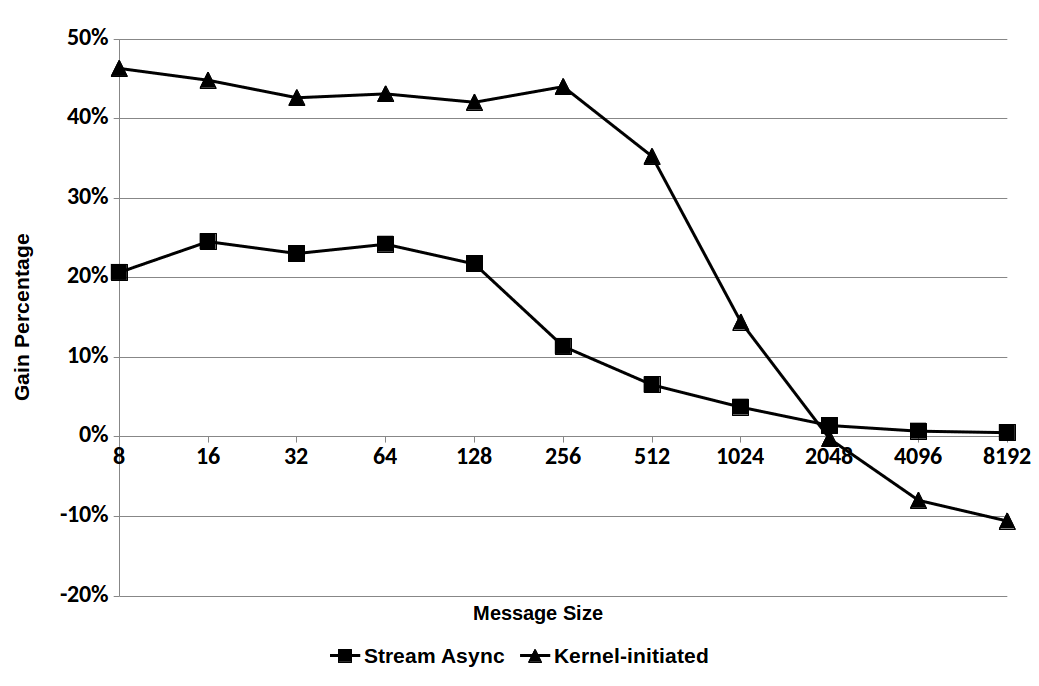
\includegraphics[scale=0.3]{gain_2dstencil_2proc_ivy.png}
%% \caption{2 processes, Asynchronous time gain, 2U Xeon Servers}
%% \label{fig:gain_2dstencil_2proc_ivy}
%% \end{figure}

%% \begin{figure}[h]
%% 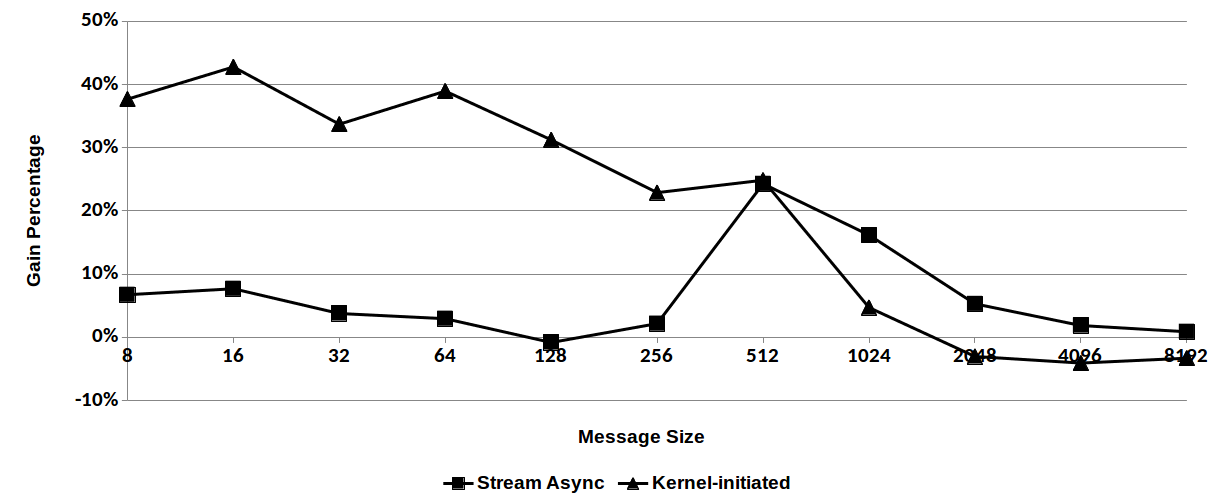
\includegraphics[scale=0.27]{gain_2dstencil_16proc_wilkes.png}
%% \caption{16 processes, Asynchronous time gain, Wilkes HPC}
%% \label{fig:gain_2dstencil_16proc_wilkes}
%% \end{figure}

% An example of a floating figure using the graphicx package.
% Note that \label must occur AFTER (or within) \caption.
% For figures, \caption should occur after the \includegraphics.
% Note that IEEEtran v1.7 and later has special internal code that
% is designed to preserve the operation of \label within \caption
% even when the captionsoff option is in effect. However, because
% of issues like this, it may be the safest practice to put all your
% \label just after \caption rather than within \caption{}.
%
% Reminder: the "draftcls" or "draftclsnofoot", not "draft", class
% option should be used if it is desired that the figures are to be
% displayed while in draft mode.
%
%\begin{figure}[!t]
%\centering
%\includegraphics[width=2.5in]{myfigure}
% where an .eps filename suffix will be assumed under latex, 
% and a .pdf suffix will be assumed for pdflatex; or what has been declared
% via \DeclareGraphicsExtensions.
%\caption{Simulation results for the network.}
%\label{fig_sim}
%\end{figure}

% Note that the IEEE typically puts floats only at the top, even when this
% results in a large percentage of a column being occupied by floats.


% An example of a double column floating figure using two subfigures.
% (The subfig.sty package must be loaded for this to work.)
% The subfigure \label commands are set within each subfloat command,
% and the \label for the overall figure must come after \caption.
% \hfil is used as a separator to get equal spacing.
% Watch out that the combined width of all the subfigures on a 
% line do not exceed the text width or a line break will occur.
%
%\begin{figure*}[!t]
%\centering
%\subfloat[Case I]{\includegraphics[width=2.5in]{box}%
%\label{fig_first_case}}
%\hfil
%\subfloat[Case II]{\includegraphics[width=2.5in]{box}%
%\label{fig_second_case}}
%\caption{Simulation results for the network.}
%\label{fig_sim}
%\end{figure*}
%
% Note that often IEEE papers with subfigures do not employ subfigure
% captions (using the optional argument to \subfloat[]), but instead will
% reference/describe all of them (a), (b), etc., within the main caption.
% Be aware that for subfig.sty to generate the (a), (b), etc., subfigure
% labels, the optional argument to \subfloat must be present. If a
% subcaption is not desired, just leave its contents blank,
% e.g., \subfloat[].


% An example of a floating table. Note that, for IEEE style tables, the
% \caption command should come BEFORE the table and, given that table
% captions serve much like titles, are usually capitalized except for words
% such as a, an, and, as, at, but, by, for, in, nor, of, on, or, the, to
% and up, which are usually not capitalized unless they are the first or
% last word of the caption. Table text will default to \footnotesize as
% the IEEE normally uses this smaller font for tables.
% The \label must come after \caption as always.
%
%\begin{table}[!t]
%% increase table row spacing, adjust to taste
%\renewcommand{\arraystretch}{1.3}
% if using array.sty, it might be a good idea to tweak the value of
% \extrarowheight as needed to properly center the text within the cells
%\caption{An Example of a Table}
%\label{table_example}
%\centering
%% Some packages, such as MDW tools, offer better commands for making tables
%% than the plain LaTeX2e tabular which is used here.
%\begin{tabular}{|c||c|}
%\hline
%One & Two\\
%\hline
%Three & Four\\
%\hline
%\end{tabular}
%\end{table}


% Note that the IEEE does not put floats in the very first column
% - or typically anywhere on the first page for that matter. Also,
% in-text middle ("here") positioning is typically not used, but it
% is allowed and encouraged for Computer Society conferences (but
% not Computer Society journals). Most IEEE journals/conferences use
% top floats exclusively. 
% Note that, LaTeX2e, unlike IEEE journals/conferences, places
% footnotes above bottom floats. This can be corrected via the
% \fnbelowfloat command of the stfloats package.


\section{Conclusion}

In this paper we presented the performance of a GPU accelerate multi-node
implementation of the HPGMG-FV benchamark using the recently introduced
NVIDIA GPUDirect Async technology.
% 
In particular, we developed an asynchronous version of a stencil
operator, that is highly used in the context of scientific and engineering
applications.  Althought communications aren't the most relevant part in
the HPGMG-FV algorithm, we reached a time gain of about 13\%.
%
Unfortunately for the moment, we had some problem during large-scale benchmarks related to the display driver released by NVIDIA along with the new CUDA 8.0 RC Toolkit.
The next step is to perform all benchmarks again up to 64 nodes on the Wilkes HPC using the most updated (and recently released) display driver 361.77.

% use section* for acknowledgment
\section*{Acknowledgment}

The authors would like to thank Sreeram Potluri for useful discussions,
and Filippo Spiga for making the Wilkes cluster available to us.


% trigger a \newpage just before the given reference
% number - used to balance the columns on the last page
% adjust value as needed - may need to be readjusted if
% the document is modified later
%\IEEEtriggeratref{8}
% The "triggered" command can be changed if desired:
%\IEEEtriggercmd{\enlargethispage{-5in}}

% references section

% can use a bibliography generated by BibTeX as a .bbl file
% BibTeX documentation can be easily obtained at:
% http://mirror.ctan.org/biblio/bibtex/contrib/doc/
% The IEEEtran BibTeX style support page is at:
% http://www.michaelshell.org/tex/ieeetran/bibtex/
%\bibliographystyle{IEEEtran}
% argument is your BibTeX string definitions and bibliography database(s)
%\bibliography{IEEEabrv,../bib/paper}
%
% <OR> manually copy in the resultant .bbl file
% set second argument of \begin to the number of references
% (used to reserve space for the reference number labels box)
\begin{thebibliography}{1}

\bibitem{IEEEhowto:kopka}
H.~Kopka and P.~W. Daly, \emph{A Guide to \LaTeX}, 3rd~ed.\hskip 1em plus
  0.5em minus 0.4em\relax Harlow, England: Addison-Wesley, 1999.

\bibitem{GPUDirect} GPUDirect family: https://developer.nvidia.com/gpudirect

\bibitem{HPGMG} HPGMG https://hpgmg.org

\bibitem{HPGMG_NVIDIA} N. ~Sakharnykh \emph{High-Performance Geometric Multi-Grid with GPU Acceleration}. \relax https://devblogs.nvidia.com/parallelforall/high-performance-geometric-multi-grid-gpu-acceleration


\bibitem{finitevolume} \emph{Finite Volume method}. \relax https://en.wikipedia.org/wiki/Finite\_volume\_method

\bibitem{fullmultigrid} \emph{Full MultiGrid method}. \relax https://en.wikipedia.org/wiki/Multigrid\_method

\bibitem{unifiedmemory} \emph{Unified Memory}. \relax https://devblogs.nvidia.com/parallelforall/unified-memory-in-cuda-6

\bibitem{ornl} \emph{ORNL Titan supercomputer}. \relax https://www.olcf.ornl.gov/titan

\bibitem{wilkes} \emph{Wilkes HPC Cambridge, UK}. \relax www.hpc.cam.ac.uk


\end{thebibliography}




% that's all folks
\end{document}


\grid
